\documentclass[12pt]{article}
\renewcommand{\baselinestretch}{1.2} 	% line Spacing
\usepackage{geometry}
\geometry{margin=1.25in}

\title{\bf \Huge{YAWYSIWYGEE} \\ \Large{Yet Another WYSIWYG Equation Editor} \\ \normalsize{Yet Another What-You-See-Is-What-You-Get Equation Editor}}
\author{John~Till}
\date{}

\usepackage[]{hyperref}
\hypersetup{
    pdftitle={YAWYSIWYGEE},
    pdfauthor={John Till},
    pdfsubject={Parsing},
    pdfkeywords={Inline Equation Editor, Typesetting},
    bookmarksnumbered=true,     
    bookmarksopen=true,         
    bookmarksopenlevel=1,       
    colorlinks=true,            
    pdfstartview=Fit,           
    pdfpagemode=UseOutlines,    % this is the option you were lookin for
    pdfpagelayout=TwoPageRight
}

\usepackage[nounderscore]{syntax}
\makeatletter
\def\gr@implitem#1<#2> #3 {%
	\sbox\z@{\hskip\labelsep\grammarlabel{#2}{#3}}%
	\strut\@@par%
	\vskip-\parskip%
	\vskip-\baselineskip%
	\hrule\@height\z@\@depth\z@\relax%
	\item[\unhbox\z@]%
	\catcode`\<\active%
}
\makeatother

\usepackage{float}                      % figure floats
\usepackage[numbers]{natbib}                     % this package allows you to link your references
\usepackage{graphicx}					% graphics package
\usepackage{fancyhdr}                   % fancy headers and footers
\usepackage[inactive]{srcltx}		 	% necessary to use forward and inverse searching in DVI
\usepackage{relsize}                    % font sizing hierarchy
\usepackage{booktabs}                   % professional looking tables
\usepackage[config, labelfont={bf}]{caption,subfig} % nice sub figures
\usepackage{mathrsfs}                   % additional math scripts
\usepackage{eufrak}
\usepackage[titletoc]{appendix}			% format appendix correctly
\usepackage{pdflscape}					% to produce landscape pages if necessary

\usepackage{amsfonts}
\usepackage{mathtools}
\usepackage{empheq}
\usepackage{pdfsync}
\usepackage{flushend}
\usepackage{verbatim}
\usepackage{mathrsfs}
\usepackage{cancel}
\usepackage{enumitem}
\usepackage{rotating} %sidewaysfigure

\usepackage{listings,textcomp,xcolor}
\lstdefinestyle{defaultStyle}
{
  basicstyle=\footnotesize,
  tabsize=2,
  captionpos=b,
  frame=lines,
  breaklines=true,
  keepspaces=true
}
% define C++ style
\lstdefinestyle{cppStyle}
{
  style=defaultStyle,
  % language related
  language=C++,
  keywordstyle=\color{violet},
  commentstyle=\color{green},
  stringstyle=\color{gray},
  showstringspaces=false,
  %otherkeywords={\#include}, % do not uncomment!
  % numbering
  numbers=left,
  numberstyle=\tiny
}
\lstset{emph={%  
    real_type%
    },emphstyle={\color{violet}}%
}%

\newcommand{\sgn}{\operatorname{sgn}}
\newcommand{\norm}[1]{\left\lVert#1\right\rVert}
%\newcommand{\bf}[1]{\boldsymbol{#1}}

\newcommand{\nomunit}[1]{%
\renewcommand{\nomentryend}{\hspace*{\fill}#1}}

%Grammar commands to use with align environment
\definecolor{terminalcolor}{RGB}{0, 185, 202}
\definecolor{nonterminalcolor}{RGB}{0, 99, 169}
\definecolor{directcolor}{RGB}{115, 65, 10}
\newcommand{\customgrammar}[1]{
\begin{align*}
#1
\end{align*}
}
\newcommand{\finishrule}{}
\newcommand{\orinline}{\;\;|\;\;}
\newcommand{\orbreak}{&\;\;\;|\;\;}
\newcommand{\terminal}[1]{\text{\textcolor{terminalcolor}{#1}}}
\newcommand{\nonterminal}[1]{\text{\textcolor{nonterminalcolor}{#1}}}
\newcommand{\direct}[1]{\text{`\textcolor{directcolor}{#1}'}}

%%%%%%%%%%%%%%%%%%%%%%%%%%%%%%%%%%%%%%%%%%%%%%%%%%%%%%%%%%%%%%%%%%%%%%%%%%%%%%%%%%%%%%%%%%%%%%%%%%%%%
\begin{document}
	\pagenumbering{alph} % this is needed to clear certain issues with the hyperref package
	\pagenumbering{roman}
	\setcounter{page}{2}

	\maketitle

	\pagenumbering{arabic}
	\setcounter{page}{1}

\section{Overview}

This project aims to create a ``what-you-see-is-what-you-get'' (WYSIWYG) editor with support for equations. An example of the editor is shown below:

\begin{figure}[ht]
	\centering
		\includegraphics[width=0.60\textwidth]{Fig/Screenshot.jpg}
	\caption{}
	\label{fig:screenshot}
\end{figure}

The editor is a Qt5 widget intended to be used in an IDE for a language with heavy mathematical emphasis.

\section{Document Data Structure: A Tree}

The basic idea of the editor is that pieces of text will be separated by typeset constructs, i.e. some mathematical notation which requires special formatting. The class to represent an alternating list of text and constructs is dubbed a ``phrase'', and is shown in Figure \ref{fig:phrase}.

\begin{figure}[ht]
	\centering
		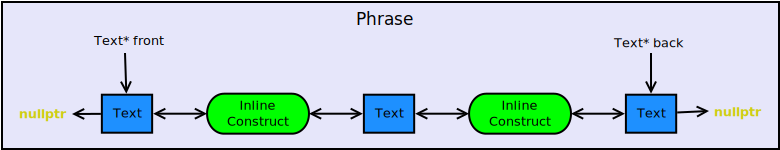
\includegraphics[width=0.90\textwidth]{Fig/Phrase.pdf}
	\caption{}
	\label{fig:phrase}
\end{figure}
The phrase will always start and end with text. Even when the text on one side of the construct is blank, we want to be able to place the text cursor there, so there will be an empty text object.
The constructs themselves will contain phrases, e.g. a fraction-construct will have a phrase in the numerator and a phrase in the denominator. Thus the document data structure is built for arbitrarily deep nesting of typeset constructs. An example of the fraction class implementing InlineConstruct is shown in Figure \ref{fig:fraction}.

\begin{figure}[ht]
	\centering
		\includegraphics[width=0.90\textwidth]{Fig/Fraction.pdf}
	\caption{}
	\label{fig:fraction}
\end{figure}

Aside from drawing the separator bar, the fraction has two child phrases for the numerator and denominator.
Thus the overall data structure is a tree. This is illustrated in the Figure \ref{fig:nested_phrase}, which shows the phrase for $x = \frac{1}{\sqrt{2}}$:

\begin{figure}[ht]
	\centering
		\includegraphics[width=0.90\textwidth]{Fig/NestedPhrase.pdf}
	\caption{}
	\label{fig:nested_phrase}
\end{figure}

When creating a whole document, there is a top level of phrases which are joined together vertically.
These phrases are aggregate members of the ``Line'' class, which also includes links to adjacent lines, and a line number as shown in Figure \ref{fig:line}.

\begin{figure}[ht]
	\centering
		\includegraphics[width=0.45\textwidth]{Fig/Line.pdf}
	\caption{}
	\label{fig:line}
\end{figure}

\section{Highlighted Selection: Document-Level State}

Selection capabilities allow the user highlight an arbitrary region of text, so that they may copy, cut, drag, delete, or perform some other action on the selection. Figure \ref{fig:complex_selection} shows this in Microsoft Word:
\begin{figure}[ht]
	\centering
		\includegraphics[width=0.50\textwidth]{Fig/ComplexSelection.jpg}
	\caption{}
	\label{fig:complex_selection}
\end{figure}

There are a variety of ways the user may change the selection. The most common (and hardest to implement) is to click within the document, drag the mouse to another point, and highlight the elements between the two points. The selection can also be changed by holding the ``shift'' key while either mouse clicking or using the keyboard.

One implication of the selection is that state must be tracked at the tree-document level. Early prototypes which had not yet considered the selection were able to treat the tree nodes as independent distributed pieces. For example, when the text cursor moved past the end of a text object, the focus is passed to the construct to the right of the text. This works well for a single cursor position, but fails when you have a selection anchor and a selection end which may span constructs and lines. The individual elements lack the information to resolve this scenario, so the selection should be implemented at the document-tree level.

The implementation can take a note from Qt5 by including a ``Document'' class to track document-level properties, and a ``Cursor'' class to handle user input at the tree level. However, unlike QTextCursor which relies on the ``textCursor'' and ``setTextCursor'' commands, the Cursor class will represent the actual cursor in the Document.

Dragging selection requires finding the connection between two arbitrary points in the tree. One first step is to find the lowest common ancestor (LCA) of the anchor point and the active point, which is the deepest shared parent of both items. Then we want to take different actions depending on whether the points are part of the same InlineConstruct, the same phrase, or belong to different lines.

\section{Undo/Redo: The Command Pattern}

Modifications to the document should be made using subclassed QUndoCommand objects. This only includes changes to the tree structure, not the selection.

\section{Save/Load/Copy/Paste: Parsing}
The typeset equations will take the form of a tree, but for the purposes of saving the document we need to define a conversion to a flat representation, and we need to parse this representation to load documents. This is also useful for copying and pasting- in the general case of using the clipboard across disconnected instances of the editor, we need a flat representation to copy to the system clipboard as well. For interactions within an editor instance, we could avoid converting to/from a string to use the system clipboard, but that is an optimization for a mature application.

The representation should be easily parsed like Lisp, and easily read. Phrases can be grouped by brackets, and inline constructs denoted by a backslash followed by an identifying character. For example, the line
\begin{align*}
x = \frac{\sqrt{2}}{2} * 2
\end{align*}
could have a flat representation shown below:
\begin{lstlisting}[xleftmargin=.33\textwidth, xrightmargin=.33\textwidth]
{x = \f{\s{2}}{2} * 2}
\end{lstlisting}

\section{Connections between Elements}

Now we understand enough of the feature set to flesh out the data structure further. Clicking on an item or moving the cursor beyond the boundaries of an item will require upward links as well as downward links. As an example, consider the equation:
\begin{align*}
\arctan(x) = \frac{1}{x^2 + 1}, \;\; i = \sqrt{-1}
\end{align*}
represented by the code:
\begin{lstlisting}[xleftmargin=.15\textwidth, xrightmargin=.15\textwidth,mathescape=true]
{arctan(x) = \f{1}{\^{x}{2} + 1}, i = $\backslash\sqrt{}${-1}}
\end{lstlisting}
This will have a data structure as shown in Figure \ref{fig:connections}.

\begin{figure}[ht]
	\centering
		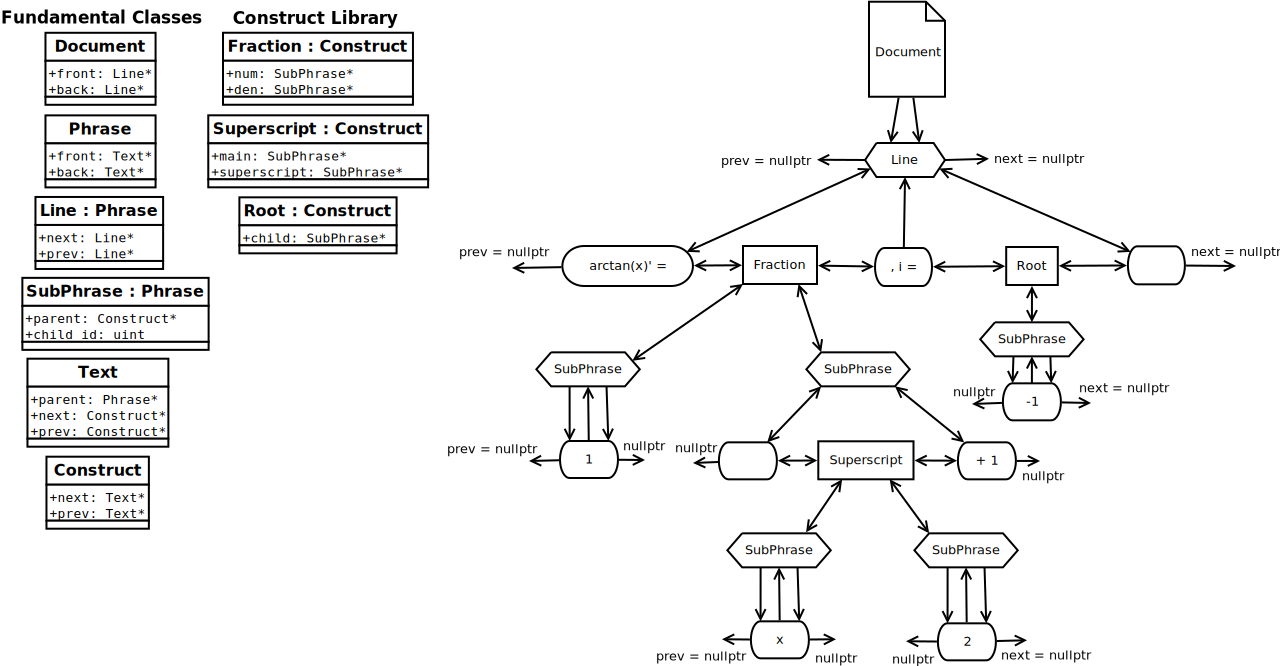
\includegraphics[width=1\textwidth]{Fig/Connections.pdf}
	\caption{}
	\label{fig:connections}
\end{figure}

\section{Layout}
We need to figure out coordinates for each element in the parent element coordinates. Elements will often be vertically aligned, but some elements will have a vertical offset, for example a superscripted element $x^2$ is vertically aligned so that the unscripted text is vertically centered. Thus elements have 3 size dimensions: the width $w$, the distance upward from the horizontal line $u$, and the distance downward from the horizontal line $d$. This is shown in Figure \ref{fig:layout_element_dimensions}.

\begin{figure}[ht]
	\centering
		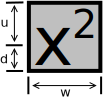
\includegraphics[width=0.25\textwidth]{Fig/LayoutElementDimensions.pdf}
	\caption{}
	\label{fig:layout_element_dimensions}
\end{figure}

Laying out elements is the sort of problem which is simple geometry, but requires drawing out the details. This section will go through each of the layouts and describe their governing equations.

\subsection{Phrase}

A phrase contains an arbitrary number of elements, which are layed out horizontally, seperated by some extra padding, and vertically aligned. This is shown in Figure \ref{fig:layout_phrase}.

\begin{figure}[ht]
	\centering
		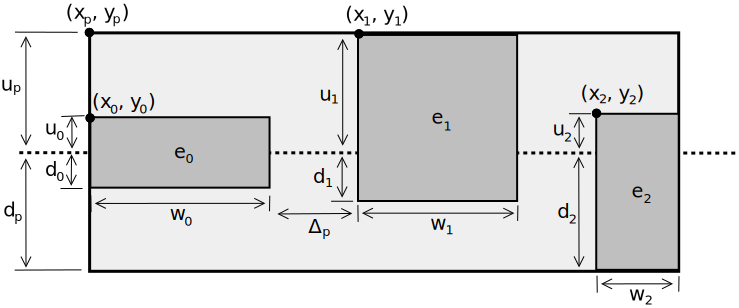
\includegraphics[width=0.8\textwidth]{Fig/LayoutPhrase.pdf}
	\caption{}
	\label{fig:layout_phrase}
\end{figure}

Let there be $n+1$ elements The independent variables are the horizontal padding $\Delta_p$ and the elements sizes $w_i$, $u_i$, and $d_i$ for $i \in [0 \;\; n]$. We need to find the phrase size variables $w_p$, $u_p$, and $w_p$, as well as the element locations $(x_i, y_i)$. We want the phrase boundaries to align with the largest element boundaries. This layout has the solution:
\begin{align*}
w_p &= w_0 + \sum_{i=1}^n \Delta_p + w_i \\
u_p &= \max_{i \in [0 \;\; n]} u_i \\
d_p &= \max_{i \in [0 \;\; n]} u_i \\
x_i &=
\begin{cases}
x_p, & i=0\\
x_{i-1} + \Delta_p, & i \in [1 \;\; n]
\end{cases} \\
y_i &= y_p + u_p - u_i
\end{align*}

\subsection{Superscript}

A superscript has a main subphrase which is horizontally centered, and an elevated script which is above the horizontal. This is shown in Figure \ref{fig:layout_superscript}:

\begin{figure}[ht]
	\centering
		\includegraphics[width=0.9\textwidth]{Fig/LayoutSuperscript.pdf}
	\caption{}
	\label{fig:layout_superscript}
\end{figure}

There is some ratio $r \in [0 \;\; 1] \subset \mathbb{R}$ defining where the furthest y-value for the bottom of the superscript box relative to the main box rise from the horizontal, $u_m$. This defines a constant $a := r u_m$. The layout has the solution:
\begin{align*}
h_s &= u_s + d_s \\
e &= \min(h_s-a, \;\; 0) \\
u_c &= u_m + e \\
d_c &= d_m \\
w_c &= w_m + w_s \\
x_m &= x_c \\
y_m &= e \\
x_s &= w_m \\
y_s &= y_c
\end{align*}

\subsection{Fraction}

A fraction construct is shown in Figure \ref{fig:layout_fraction}. There are parameters $\Delta_v$ and $\Delta_h$ to specify vertical and horizontal buffers from the fraction bar.

\begin{figure}[ht]
	\centering
		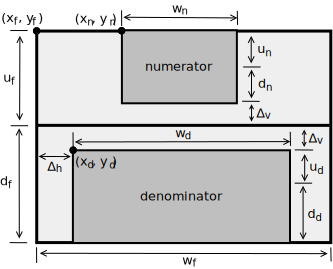
\includegraphics[width=0.8\textwidth]{Fig/LayoutFraction.pdf}
	\caption{}
	\label{fig:layout_fraction}
\end{figure}

This layout has the solution
\begin{align*}
w_f &= \max(w_n, \; w_d) + 2\Delta_h \\
u_f &= u_n + d_n + \Delta_v \\
d_f &= u_d + d_d + \Delta_v \\
x_n &= x_f + (w_f - w_n)/2 \\
y_n &= y_f \\
x_d &= x_f + (w_f - w_d)/2 \\
y_d &= y_f + u_f + 2\Delta_v
\end{align*}

\subsection{Root}

Figure \ref{fig:layout_root} shows the problem of laying out a square root. There is only one child element here; the problem is to define how the root symbol scales as the child size changes.

\begin{figure}[ht]
	\centering
		\includegraphics[width=0.4\textwidth]{Fig/LayoutRoot.pdf}
	\caption{}
	\label{fig:layout_root}
\end{figure}

Probably a good rule is that the line $\overline{p_2p_3}$ has a constant slope, and that the overbar be at a constant offset above the child.

\subsection{Matrix}

One of the harder layout problems is two-dimensional data. Figure \ref{fig:layout_matrix} shows a matrix layout.

\begin{figure}[ht]
	\centering
		\includegraphics[width=0.6\textwidth]{Fig/LayoutMatrix.pdf}
	\caption{}
	\label{fig:layout_matrix}
\end{figure}

We begin
\begin{align*}
W_j &= \max_i w_{i,j} \\
U_i &= \max_j u_{i,j} \\
D_i &= \max_j d_{i,j} \\
x_{i,0} &= (W_0 - w_{i,0})/2 \\
x_{i,j} &= (W_j - w_{i,j})/2 + j\Delta_h + \sum_{k=0}^{j-1} W_k \\
y_{0,j} &= U_0 - u_{0,j} \\
y_{i,j} &= U_i - u_{i,j} + i\Delta_v + \sum_{k=0}^{j-1} U_k + D_k
\end{align*}

Let there be $n+1$ rows and $m+1$ columns.
\begin{align*}
w_a &= m\Delta_h + \sum_{j=0}^m W_j \\
h_a &= n\Delta_v + \sum_{i=0}^n U_i + D_i \\
u_a &= d_a = h_a / 2
\end{align*}

Also need to account for offset between array coordinates and matrix coordinates. The offset could be constant, or could be a function of $w_a$ and $h_a$.

\section{Automatic Syntax Formatting}

The editor could also benefit from features of code editors such as syntax highlighting, parenthesis matching, and autocompletion. I fear that parenthesis matching may be complicated by the tree structure. I want to allow the user to define syntax rules, so that for example if a certain identifier is determined to be a matrix by a parser, that identifier may be bolded wherever it occurs.

Of course, it should also be possible to change the editor font and color scheme.

\section{Unicode}

The editor will include functionality to insert relevant mathematical unicode symbols with word substitutions and GUI elements. For example, typing ``$\backslash$pi'' in a Word equation and hitting space after will result in the symbol `$\pi$' being substituted. Of course Word also has drop-down menus with a table of symbols which may be clicked to insert, and this feature should be standard in any equation editor.

\section{Library of Constructs}

The editor will need to include quite a few mathematical notations, including:
\begin{itemize}
\item Fractions
\item Roots
\item Integrals
\item Matrices
\item Superscripts, subscripts, other scripts
\item Summations, products, other big operators
\item Dots, overbar, hyphen, other accents
\end{itemize}
Many of these methods merely need to draw a symbol and position child phrases appropriately. However, there are a few complications which will need to be handled in an adhoc way. For example, matrices have a variadic size. Also, the phrase in a superscript should be a smaller fontsize than the text outside of it. This effect should nest to at least two levels, although eventually it is reasonable to have a minimum font size in deeply nested scripts.

Aside from mathematical constructs, we might also want tables and pictures.

\end{document}
